%%%%%%%%%%%%%%%%%%%%%%% file template.tex %%%%%%%%%%%%%%%%%%%%%%%%%
%
% This is a template file for The European Physical Journal H
%
% Copy it to a new file with a new name and use it as the basis
% for your article
%
%%%%%%%%%%%%%%%%%%%%%%%% Springer-Verlag %%%%%%%%%%%%%%%%%%%%%%%%%%
%
\documentclass[epjH]{svjour}
%
\usepackage{graphicx,subfig,amssymb,bbm,wrapfig}

%
\newcommand{\noun}[1]{\textsc{#1}}

\begin{document}
%



\title{Discrete Choice Models for Bike-Sharing Transportation Systems}
\subtitle{Inference of Discrete-Choice parameters by coupling Statistical Analysis and Agent-based Modeling}
\author{Juste Raimbault\inst{1}\inst{2}\fnmsep\thanks{\email{juste.raimbault@polytechnique.edu}} }
%
\institute{Graduate School, Ecole Polytechnique, Palaiseau \and LVMT, UMR-T 9403 IFSTTAR, Champs-sur-Marne}
%



\abstract{
The realization of developed user surveys, generally used to elaborate and calibrate transportation systems models with an aim of improvement of the level of service, is heavy to implement and has a certain cost. We propose an alternative method to obtain similar results, combining poor quality survey data and raw data on system evolution, fed into an hybrid statistical and agent-based model. The method is described on the particular case of bike-sharing transportation system for which surveys are destined to parametrize discrete choice models. We work on the real system of Paris (V�lib) with 1 year of recent data on system dynamics. It should be easily generalized to other kind of systems and research questions, as the core principle of hybrid modeling has already been well documented in the literature (see e.g. recent works in archeology \cite{crabtree2012modelling}). We find that we can retrieve discrete choice parameters indirectly by parametrizing and calibrating an agent-based model including discrete choice models at finest granularity, and propose a novel method to assess the robustness of the inference.
} 



%
\maketitle
%




\section{Introduction}

\subsection{Context}

Discrete Choice Modeling has been widely used in Transportation Science, showing both a powerful theoretical framework in formalizing crucial but fuzzy components of a social systems (i.e. choices of irrational agents) and mature applications in transportation systems management with dedicated frameworks (such as Biogeme \cite{bierlaire2006biogeme} software) including e.g. mode share or route choice predictions, adapted pricing solutions, more accurate planning of public transport, or other application detailed in \cite{ben1999discrete}.

With the rise of novel transportation modes in cities, a precise knowledge of potential user behavior and pattern of system use is necessary during conception and management phases. Therefore the use of discrete choice models can be a powerful asset. We are particularly interested in Bike-sharing transportation systems, which have been presented as an ecological and user-friendly transportation mode and performs a good complementary with classic public transportation modes (\cite{midgley2009role}). Although the direct positive impact on public health is not systematically proved and the modal share report does not necessarily occurs from polluting modes as the recent review in  \cite{fishman2013bike} highlighted, we follow \cite{o2013mining} on the fact that the success of such systems in Europe and its current transposition in other regions of the world such as China (\cite{liu2012solving,geng2009bike}) or the United States (\cite{gifford2004will}) is an acceptable reason for helping its development by the study of its mechanisms and possible measures to improve its level of service.
Our context is therefore the use of discrete choice models at small granularity (user) to investigate behaviors and mechanisms in a given bike-sharing system .We focus on the Paris case, and qualitative conclusions do depend on cultural and geographical frame \cite{o2013mining}, but their extension or generalization is not our purpose here. However, as the applied method is quite generic, that aspect of our work could be transposed to other systems or fields in further works.

\subsection{Project Description}

As the final result of this scientific project is the result of many contradictory steps and concrete difficulties to follow the initial sketch of plan, in particular the impossibility to realize the expected questionnaire and gather the data that would have allowed a fine Discrete Choice modeling, the general plan may not seem natural at first sight, thus we propose to explicit a rough temporal timeline of research questions that drove the project, and its link to that final form. Sequentially, we explored the following problematics :

\begin{enumerate}
\item Conceive and realize a precise survey, in order to estimate discrete choice models, particularly on user choices done when taking or dropping a bike.
\item Insert the discrete choice model in an existing (but basic) agent-based model for Paris bike-sharing system described and explored in \cite{raimbault2014user}.
\item Because of practical issues, initial survey that was expected to be revealed preferences and with some characteristics, was replaced by a stated preferences survey with more simple characteristics and attributes.
\item The problem became : how to use this poor quality data ? Can we however answer the initial question ?
\item We elaborated the calibration method to infer DC parameters and partially tackle it. Core results became then more of methodological than practical type.
\end{enumerate}

We can mention an explored direction that is not reported here because of issues in implementation and low priority regarding research question. We tried to proceed to a crossed systematic review on all bike-sharing and discrete choice literature, using a novel method which provide a precise dynamic scientific taxonomy of the fields (general method introduced and applied in~\cite{chavalarias2013phylomemetic}). Its advantages are that it provides information on the evolution of the field and therefore allows in general to make unexpected connections between concepts or fields, suggesting potential research directions. A sketch of Java implementation using Graphstream library for dynamic graph handling~\footnote{http://graphstream-project.org/}. Text-mining of the corpus of citations extracted from Web of Science was done thanks to the online tool provided by authors~\footnote{http://manager.cortext.net/}. Unfortunately the method was not successful so we do not develop it here as it has in that state of things few relation to our purpose.

Note that all source code and data used in the project are openly available on the Github repository of the project~\footnote{at https://github.com/JusteRaimbault/DiscreteChoicesBikeSharing}. It is a crucial point for practice of Open Science and reproducibility \cite{ram2013git}.

We describe in a first section the different data collection processes which were a considerable part of our project. We then present Discrete Choice Models proposed and estimated. Sec. 4 describes statistical analysis of raw data, including a case study on missing data inference. Sec. 5 describes the agent-based model and its discrete choice extension, used in the last part to infer discrete choice parameters through model calibration. We conclude by proposing a method to study stability of multidimensional calibration.




\section{Data Collection}
\label{sec:data}


\subsection{Discrete Choice Questionnaire}

In order to collect data for Discrete Choice modeling through surveys, we conceived and implemented a generic web-application for questionnaire administration, which could be used either for direct web survey or during terrain survey. Because of the uncertainty on the form of the questionnaire and on the feasibility of the survey, we proposed a totally adaptable application allowing variable questionnaire structure. Thanks to a restricted access interface, an administrator can create a questionnaire, specifying general description characteristics, attributes, choices, number of output scenarii , type of experimental design. Structure is stored in static tables in database, whereas a dedicated dynamic table is created to store user answers. Questionnaire administration can be done by an authorized user (personal survey) or by anonymous users on the web, for which security requirements (in particular an anti-bot captcha) were added. Furthermore, a data export module allows to export data directly to the specific Biogeme format (csv-like), given a filter specification file (for dummies formatting e.g.).

The application was implemented as a server-side php-application, including a large use of jQuery and Ajax request that allow lightweight navigation and a simplified architecture of contents and utilities pages. Database is efficiently managed by a classic Mysql base (since expected data size stays small, at least always smaller than 1Mo), exploited through current php drivers (PDO). It is installed on a web server, implying security management because of public access of a part of the questionnaire. For reproducibility sake, platform code is Open Source~\footnote{available at https://github.com/JusteRaimbault/Questionnaire}, as for data available at the public export URL given in the following.

Concerning data export~\footnote{Data export public URL : http://37.187.242.99/Questionnaire/php/utils/export.php}, a particular treatment was needed as there is no necessarily direct correspondence between raw variables and Discrete Choice Models variables, for example in the case of dummy variables. Therefore, a text file declaring filter format is needed under the following format : each row is an output variable (column in output .dat file) and follows the template [BIOGEME\_VARIABLE\_NAME ; BASE\_VARIABLE\_NAME ; BASE\_VALUE ]. If BASE\_VALUE = NULL, value is unchanged (quantified variables). In an other case, output is a dummy variable which is 1 if and only if value of the record correspond to the provided value. For more flexibility, we also implemented a mapping which allow to apply a function to quantitative variables (formatted by BASE\_VALUE=NULL :v1-f(v1) :v2-f(v2) :... :vn-f(vn)).

This platform allowed to test experimental questionnaires, to realize the simplified survey and to quickly generate data used in the second discrete choice model described before.


\subsection{Raw Data on System Dynamics}

\paragraph{Type of data}

We also collected raw data data for the statistical analysis and parametrization of the final model. They are public available data (open data) from the bike-sharing system of Paris (``V'Lib''), provided by the operating company in direct time on a dedicated website (url \texttt{http://api.jcdecaux.com}, for which the format of request is specified on \texttt{developer.jcdecaux.com}). It provides only the status of docking stations at the request time so we had to automatize the data collection process on a large time period in order to have significant time-series. Process is detailed in the following.

We chose to gather such kind of data first because the obtention of more precise data from the company can raise several problems such as confidentiality issues or more constraining for our research, lead to an lack of independence in the design of the modeling process, since most of the time delivering of data had its price that is at least answering to some question asked by the company. Secondly, we argue that our experience will be one way of testing the possibilities and limits of open data: if the public provided data can lead to relatively good results compared to what can be obtained with a larger set. However, if our research process becomes quickly limited by the lack of precision or diversity in the data, that will bring one essential question on front, that is that open data does not necessarily means freedom not exhaustivity, and that the control of the provided data can implicitly be highly dangerous for the global opening process. On that point, we follow \noun{Banos} in \cite{banos2013HDR} when he argues that a necessary condition of an open scientific cumulative process is a total transparency in the methods and an exhausting sharing of implementations of models of simulation and of data. Furthermore we wanted to avoid any risk of implicit reporting spin since it stays a major issue today for the quality of research as it is claimed by \noun{Ravaud} \& \textit{al}. in \cite{boutron2010reporting}. The purpose of data sharing by the company in our case was surely,
because of the nature of the available data, i. e. only current time
stations status, nothing more than current time information and mapping.
However, we will see that we can use them for statistical analysis
and obtain quite good results.

\paragraph{Data collection process}

A script requesting current data to the API and saving it into a file
have been written and scheduled each 5 minutes on a remote server
(we did not choose finer temporal granularity for a material reason,
because the size of data becomes quickly huge and storage becomes
then an issue). Data on remote server is then zipped everyday for
storage purpose. When needed we download the files and process them
with R using \cite{couture2013rjson} in order to store them locally
on a reduced form (csv) that can be called directly by our data processing
algorithms. Note that it would have been more logical to process the
data remotely and store them under the reduced form but technical
reasons were an obstacle (in particular the installation of R on the
remote machine). We also extracted from extensive files static information
such as numbering and coordinates of docking stations, what have
been useful after for example to create a geographical file for map
drawing with \cite{keitt2011rgdal}. Fig. 1 shows a flowchart of the
data collection and primary processing process. We collected data
for all Paris during around 3 month, following statistical analysis
are done on these data.

\begin{figure}[[h]
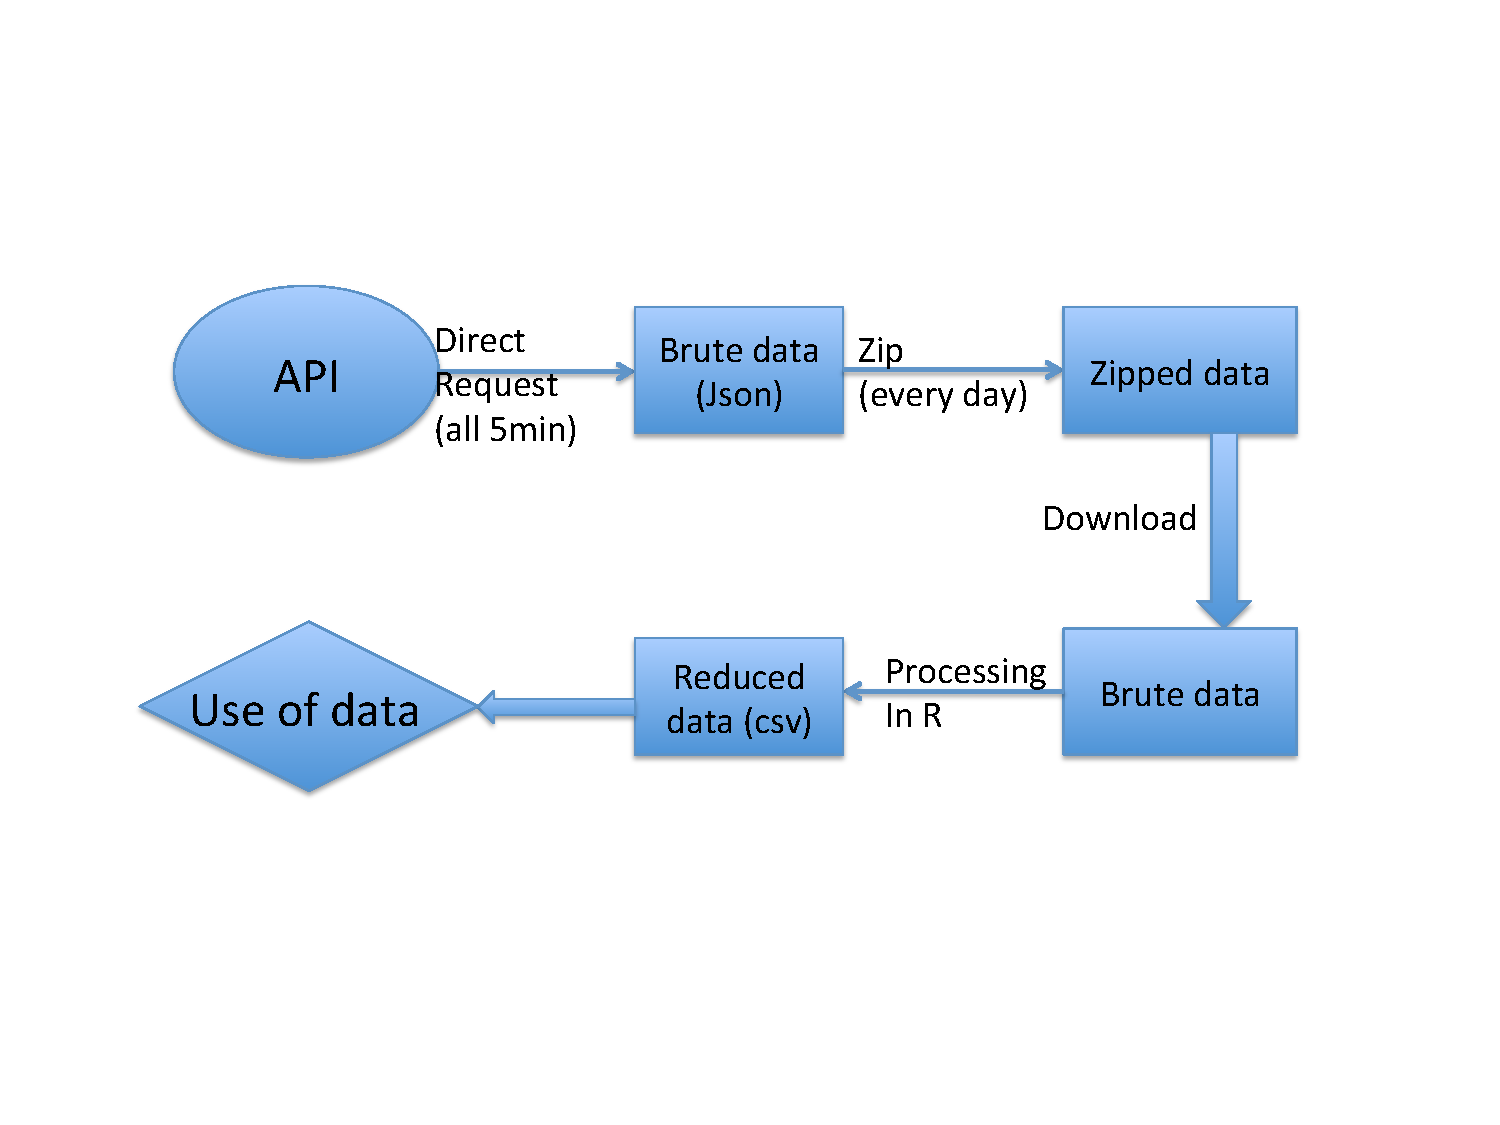
\includegraphics[bb=0bp 100bp 720bp 540bp,scale=0.45]{data}
\caption{Flowchart of raw data collection process}
\end{figure}






%%%%%%%%%%%%%%%%%%%%
%% Discrete choice modeling
%%%%%%%%%%%%%%%%%%%%

\section{Discrete Choice Modeling}

\subsection{Towards a precise discrete choice behavioral model}

The initial aim of our project was to collect survey data to estimate precise behavioral discrete choice models for bike-sharing users. Many factors of choice had to be considered, implying nested models. Among others, they included modal choice, and in the bike-sharing nest, route choice, destination choice, docking station choice and redirection procedure in the case of an adverse event (full station). A precise modeling of user behavior would have been essential for a precise parametrization of an agent-based model of bike-sharing. Indeed, rules where decisions are involved and basic probabilities are used in a root model, discrete choices are the key for a step of desegregation further.

Table~\ref{tab:1} give a first sketch of revealed preference questionnaire, designed to answer the above questions. It could not be tested nor implemented, thus its use was nothing more than the inspiration of the simplified stated preferences survey described below.

\begin{table}[h]
\centering
\caption{Proposed detailed survey for behavioral Discrete Choice Models.}
\label{tab:1}  
\begin{tabular}{lll}
\hline\noalign{\smallskip}
Category & Variable & Observations  \\
\noalign{\smallskip}\hline\noalign{\smallskip}
Survey context & Localization & Determined by geolocalization  \\
 & Day, time &  \\
 & Weather & Collected automatically \\
 & Remarks & \\
 Socio-economic profile & Age & Determine relevant age classes \\
 & Occupation & idem \\
 & Income & Delicate question \\
 & Household infos & Size, residential localization \\
 Transportation profile & Motorization & Personal and household \\
 & Public transport subscription & Range \\
 & Frequent O/D & By mode and motive \\
 & Frequency & idem \\
 & Mean distance & idem \\
 & Bike-sharing subscription & \\
 & Specific bike-sharing O/D &\\
 & Car-sharing subscription &\\
 & Car-sharing O/D & \\
 Bike-sharing profile & Typical schedule of use &\\
 & Frequencies & Weekly, monthly \\
 & Typical week & \\
 & Mean traveled distance & \\
 & Factor of choice & Subjective \\
 & Route choice procedure & idem \\
 & Concurrent mode &\\
 & Complementary mode & \\
 & Walking distances to bike & Origin and Destination\\
 & Use of electronic device & Type, moment, purpose\\
 & Subjective impression & System, level of service, typical behavior \\
 & Docking stations choice & Experience, expected charge, proximity, random\\
\noalign{\smallskip}\hline
\end{tabular}
\end{table}


\subsection{Simplified incomplete model}

As described in introduction, practical reasons made the initial survey impossible to realize, and a simpler stated preference survey with relatively few answers was imposed by external constraints. The conception and realization was done in a joint student project \cite{bourcet2014vlib} which beneficed from the developed online interface described above. Following the general context of our study, interesting results from that modeling that we reuse are potential intervals for some discrete choice parameters, allowing an efficient bootstrap of calibration procedure.

Let review briefly the structure of the model and main results.

Accounted socio-economic variables of users are
\begin{itemize}
\item age
\item professional categorization
\item regular user
\item average distance to public transport
\end{itemize}
We also consider weather as a characteristic as it will be taken as exogenous in stated scenarii.

Choices are simplified as they are only between bus and bike-sharing (comparable ranges and speeds). Attributes of choices are, with respective notations : travel distance $D$, expected travel time $t$, time to find a bike $t_B$, time to drop a bike $t_D$, bus delay $D$ and bus comfort $C$. Attributes levels are chosen with 3 level for each discretized attribute (from $t_B$ to $C$).

Scenarii are given following a Random Experience Plan (with deletion of dominated scenarii), which thanks to the 150 data rows collected gave a reasonable random sampling of the space.

Discrete choices utilities are linear in the simpler model estimated : denoting $X_{bus}$ or $X_{bike}$ attributes and characteristics of each choice, we write $U_{bus}=\sum{\beta_{X_{bus}}X_{bus}}+\varepsilon_1$ and $U_{bike}=\sum{\beta_{X_{bike}}X_{bike}}+\varepsilon_2$.

%% Precise used result :: confidence intervals for parameters.
Models were estimated with Biogeme and robust value were found for most of parameters, with expected signs. For the following, important results are the confidence intervals : $\beta_D \in [-0.06,0]$ and $\beta_{t_{B}}\in [-0.25,-0.15]$. 


\section{Statistical Analysis}

\label{sec:stats}



As explained before, the central question of our project has quickly become how to deal with bad quality data, in two sense : not necessarily expected variables observed (realization of an other questionnaire) and poor statistical robustness because of a small number of answers (around 150 rows in database).
Therefore, a statistical analysis appeared to be the best way to
\begin{itemize}
\item Test for methods to fill missing rows (handling of missing data)
\item Understand underlying data structure and therein system behavior
\item Propose missing variables inference
\end{itemize}
the third point being crucial for the following as it allows to parametrize the agent-based model through Origin/Destination inference. This paragraph follows these three aspects as a plan.


\subsection{Handling Missing Data : a case study}

%% Explanation / intro

Facing the issue of poor quality data, we explored ways to tackle missing data. We studied more precisely some techniques as a case study. We comment on recent progresses done to compare different methods of handling missing data, that are called imputation methods for missing baseline data. Such methods are particularly scrutinized by statisticians working in Therapeutic Evaluation but methods and results can be easily generalized to any domain involving statistical models on potentially incomplete data. We focus on \cite{crowe2010comparison} and  \cite{mitra2010comparison} that try to compare methods for imputation, and the consequences of choices on final results of evaluation of treatment effect.

Missing data in dataset are an essential problem to tackle in statistical analysis of treatment effect. One does not simply remove patients with missing data since it brings more bias and leads to unbalanced data at it is explained in the discussion of \cite{crowe2010comparison}. First methods for imputation of baseline data were proposed by \noun{Rubin}\cite{rubin2009multiple}. Multiple imputation methods are compared between themselves (and with mean imputation and with results with no missing data in the binary outcome case). The missing values in the set of values $\mathbf{X}$ are filled through statistical model (that differs between the methods), and it is done $m$ times to obtain $(\mathbf{X}{}_{i})_{1\leq i\leq m}$ completed datasets from which propensity scores are calculated.

\paragraph{Filling missing data}
The objective of the first work with binary outcome (death or not) by \noun{Crowe} \& \textit{al}. in \cite{crowe2010comparison} is
to compare through numerical simulations the influence of the model
chosen to proceed to multiple imputation on the bias and variance
(confidence interval in fact) of the results.
The method for numerical simulation is:
\begin{itemize}
\item Random normal generation of 6 explanatory variables and assignment to $\mathbf{X}$
\item Assignment of treatment following a logit model controlled only by the first variable (with a variable parameter)
\item Assignment of treatment effect also following a logit, depending on both treatment and the first variable (also variable parameters)
\item Suppression of data (or creation of missing data in other terms), for some ``completely at random'', i. e. setting a given proportion of values to random uniform distributed values. If one rows is set to missing data, the two following variables will also have missing data on that row. Then some data are suppressed ``at random''; this time the data supposed to be suppressed will be if it is positive (so it depends on the value of the variable).
\item Then all possible methods for imputation are tested:

\begin{itemize}
\item with complete data (as a comparison)
\item with treatment mean imputation (no multiple imputation, that mean
replacing missing data by the mean)
\item multiple imputation using as controls in the regression model for
imputation only explanatory variables
\item multiple imputation using also treatment
\item multiple imputation using explanatory variables, treatment and outcome
\end{itemize}
\item bias and confidence intervals are estimated in each case
\end{itemize}
The main conclusion is that the best multiple imputation method was
the one controlled by explanatory variables, treatment and outcome.
It is also obvious to note that ``complete data'' method (i.e. deleting
the row with missing data) leads to less bias but to strong variance,
so quite less significance of the results on treatment effect, as
we stated in introduction. Although the multiple imputation brings
bias compared to a scenario with all data (called the ``gold scenario''
in the paper), it is sure that if baseline data are missing, best
choice is to use multiple imputation with controls by variables, treatment
and outcome.


\paragraph{Sensitivity of estimators to missing data}

An other way to tackle the question is to directly look at the sensitivity of estimators for mean treatment effect, noted $\tau$, on missing data and methods used to reconstruct it. Indeed, two approaches are possible (called the Within and the Across approach). The Within is called like that because estimates first treatment effect in each completed dataset by matching and then estimates the treatment effect by taking the mean of all estimated treatment effect, so the matching is done ``within'' each completed dataset. In the Across method, a mean propensity score is first calculated from all propensity scores of completed datasets and then the matching is done on that mean.

Formally, if we note $\mathbf{e}(\mathbf{X})$ the vector of propensity scores for data $\mathbf{X}$ and $\tau(\mathbf{e})$ the corresponding estimated treatment effect through matching, we have the estimator in the Across approach given by
\[
\hat{\tau}_{Ac}(m)=\tau\left(<\mathbf{e}(\mathbf{X}_{i})>_{1\leq i\leq m}\right)
\]
whereas the estimator in the Within approach is
\[
\hat{\tau}_{Wi}(m)=<\tau(\mathbf{e}(\mathbf{X}_{i})>_{1\leq i\leq m}
\]
One can have a generalized point of view to gather both approach, by considering the extended Across approach: if $(\hat{\tau}_{Ac}^{(j)}(m))_{1\leq j\leq r}$ are $r$ realizations of an estimator in the Across approach, we can take the mean and define the generalized estimator
\[
\hat{\tau}(m,r)=<\hat{\tau}_{Ac}^{(j)}(m)>_{1\leq j\leq r}
\]
that is quite practical since we obviously have $\hat{\tau}_{Wi}(m)=\hat{\tau}(1,m)$
and $\hat{\tau}_{Ac}(m)=\hat{\tau}(m,1)$.

\begin{itemize}
\item First, artificial data with two covariates are simulated with Logit models both for treatment distribution and indexes of missing data, and different parameters for the logit for treatment assignment are tested (i. e. treatment assignment depending on only one covariate, and one both with equal weights). Bias and variance are estimated in each case.
\item The comparison is also done on real data for different values of $(m,r)$ in the generalized estimator. An heuristic for the selection of the best values for the couple is proposed, what can be considered as a compromise between the two initial approaches.
\item Theoretical formulation of limit variance estimators are proposed for both cases but they are not used. The development and study of such estimators is pointed out as a key-point in further research.
\end{itemize}
The main results to this second question are that, for artificial data, across method gives smaller bias than within method in the case where the covariate with most of missing data was most influent in treatment assignment, although variances were smaller for within method (with quite same mean square errors). In other parametrization of logit models, the two estimators gave quite the same results. Following the work done on genuine data, they finally advise to use generalized estimator, and use the heuristic for finding best values of $(m,r)$ that can lead to the best compromise between bias and variance values.










\subsection{Data-mining of raw data}


\subsubsection{Data visualisation}

Many basic means for a global visualization of data behavior are available
such as the ones proposed in \cite{o2013mining}, so we won't go too
much into detailed representation since it is not the first purpose
of our study. Note that this step is however essential, especially
during the elaboration of algorithm and the choice of methods for
statistical treatment.

To have an idea of the cyclic character of daily mobility patterns,
we can plot the total number of available bikes at docking stations
against time. If we suppose the total number of bikes constant over
the time duration of the plot, what seems reasonable even on the
all time period our data cover (even if there are surely variations
because for example of bike reparations, they are surely negligible
regarding the total number of bikes, which is around 15000), this
plot is exactly the complementary of the quantity of current travel
as a function of time, what allows to visualize mobility trends.
Fig. 2 shows the obtained curve that fits the expected results, showing
in particular the distinction between week days and weekends.

\begin{figure}
\centering
\resizebox{0.75\columnwidth}{!}{
\includegraphics[scale=0.45]{/Users/Juste/Documents/ComplexSystems/CityBikes/Results/Visu/availableBikes}
}
\caption{Quantity of total available bikes over a week. We observe the typical
patterns of the daily mobility, with two minima corresponding to morning
and evening affluence. The two day in the middle correspond to saturday
and sunday since the time-serie begins on a wednesday. These weekend days
present only one minimum, what is logical (no affluence in the morning)
and confirms the results of other studies.}
\end{figure}

We can also for example draw maps for the understanding of spatial
patterns in system use. One can expect for example to see distinction
in time between residential and activity areas for the quantity of
available bikes in stations. This allows to visualize global and local
heterogeneity patterns. Fig.~\ref{fig:heatmaps} shows an example of such maps on a
particular district.

\begin{figure}
\label{fig:heatmaps}
\subfloat[Midnight]{\includegraphics[scale=0.45]{/Users/Juste/Documents/ComplexSystems/CityBikes/Results/Views/lfmidnight}}\\
\subfloat[Midday]{\includegraphics[scale=0.45]{/Users/Juste/Documents/ComplexSystems/CityBikes/Results/Views/lfMidday}}
\caption{Examples of heatmaps at two different moments of the day for the district
of Chatelet. The color indicates, from green that corresponds to an
empty station, to red to a full one, number of available bikes. Since
it is a working district and not residential, stations in the center
are overloaded during the day but empty during the night as expected.}
\end{figure}



\subsubsection{Extraction of patterns}

A first step in the treatment of data is to extract typical patterns
in use of the system. In \cite{vogel2011understanding}, data-mining
techniques, and especially clustering of activity profiles, are used
to extract typical patterns in station use. We propose to use similar
methodology in order to identify typical overall day profiles and
classify them. We expect to be able to differentiate weekdays from
week-ends for example, but also see the influence of climate on use
patterns. The clustering of time-series offer an alternative for a
predictive model, as the cyclic model proposed in \cite{borgnat2009modelisation,borgnat2009studying}.


A day is exhaustively represented by the time-series, defined on all
the stations of the system $s\in S$, and on a discrete time sample
$T=\{0,\tau,...,N\tau\}$ (with $\tau$ time step of the data, 5min
in our case), $(b(s,t))_{s\in S,t\in T}$ of available bikes at each
stations. Each station has a maximal capacity $c(s)$ that allow to
define the number of free parking places $p(s)=c(s)-b(s)$ and the
load factor which can be more convenient to work with since it is normalized
$lf(s)=\frac{b(s)}{c(s)}$. The overall clustering process first aims
to reduce the dimension of the representation of a day without loosing
majority of information, and then to be able then to classify days
and make predictions on the day characteristics from its data.


First the dimension is reduced through a sampling process that can
be seen as a projection from the space of complete time-series to
a space of smaller dimension. If $\varphi \in \mathbb{N}^{\mathbb{N}}$
is a extraction then the sampling is defined as the canonic projection
$\mathcal{S}:\mathbb{R}^{\left|T\right|\left|S\right|}\rightarrow\mathbb{R}^{\left|\varphi(T)\right|\left|S\right|}$.
The question of the value of the time step for sampling is important.
We tried for many values and looked at the possible loss of information
through the evolution of clustering coefficient regarding number of
clusters. It appeared that we had still good precision for large time
steps such as one hour. See fig.~\ref{fig:info} for more precision on the influence
of sampling step.


\begin{figure}
\label{fig:info}
\centering
\subfloat[Clustering coefficient as a function of cluster number for different
values of sampling step. The more blue the curve is, the more sampling
step is large. If the curve goes faster to 1, that means that points
are less distinct and that statistical distribution contains less
information. We observe a jump that is quantified in (b).]{\includegraphics[scale=0.3]{/Users/Juste/Documents/ComplexSystems/CityBikes/Results/Clustering/clusterNumber}}
\hfill{}\subfloat[Plot of the value of the clustering coefficient for k=2 (red) and
k=3 (green), as a function of sampling step. We see the significative
loss of information around a step of 400 minutes, which should correspond
to the disappearance of pics in the curve, since they contribute significantly
to the quantity of information.]
{\includegraphics[scale=0.3]{/Users/Juste/Documents/ComplexSystems/CityBikes/Results/Clustering/infoLoss}}
\caption{Influence of sampling interval on quantity of conserved information
in the clustering process.}
\end{figure}


We proceed then for each day to a k-means algorithm on the sampled
time-series (as described in \cite{warren2005clustering}), in order
to reduce more the dimension needed to represent a day. Intuitively,
that corresponds to a classification of stations according to their
``profile''. We take in practice 20 clusters, what allows to divide
by 100 the dimension. The final step is to cluster the representations
of the days for establishing a classification of days. With two clusters,
one expect to isolate weekdays from weekends, although k-means can
lead to bad results if cardinal of clusters appear to be imbalanced.
In our case it worked quite well and we were able to reproduce that
distinction. However, a finer distinction (e. g. between rainy and
shiny days) was not possible and some work on a more specialized clustering
algorithm (k-means is very general) would be needed to obtain more
precise results. Fig.~\ref{fig:clustering} shows the comparison between real curves of
available bikes and predicted curves by the clustering algorithm.


\begin{figure}
\label{fig:clustering}
\centering
\subfloat[Curves of available bikes for all day of the week. Week days are superposed
and correspond to the curves with two pics. the green and the blue
curve are respectively saturday and sunday.]{\includegraphics[scale=0.25]{/Users/Juste/Documents/ComplexSystems/CityBikes/Results/Clustering/week}}
\hfill{}\subfloat[Theoretical predicted curves for two clusters. As expected, we distinguish
week days (red curve) from weekend (blue curve), according to the
real curves.]{\includegraphics[scale=0.25]{/Users/Juste/Documents/ComplexSystems/CityBikes/Results/Clustering/curves}}
\caption{Results of clustering process for classification of days: distinction between weekends and week days.}
\end{figure}












\subsection{Inference of O/D fields}

The core part of statistical analysis within the all project is indeed the inference of unknown variables, that are probability distribution of Origin and Destination fields of users, needed for model parametrization. Note that this question has its own scientific interest and has already been tackled in economic geography and transportation geography (see \cite{leurent2006modelisation} e. g.).

%% Subsection on GWR

\subsubsection{Geographically Weighted Regression}

The method used for inference is indirectly linked to a powerful approach of geographical statistics, called Geographically Weighted Regression (GWR). It was introduced relatively recently by \noun{Bronson} in order to integrate neighborhood effect in statistical analysis, i. e. integrate the spatial dimension in data analysis \cite{brunsdon1998geographically}. The core feature is to build from data an hypothetical continuous spatial field by non-parametric estimation (kernel mixture) and proceed to statistical analysis such as regressions on sub samplings of this field. Kernel choice can be function of euclidian distance (gaussian, quadratic) but not necessarily (e.g. cultural or income distance) \cite{lu2011geographically}. Kernel size plays a central role in final results, and calibration procedures by cross-validation were also developed \cite{brunsdon2002geographically}. All current methods linked to GWR are implemented in a R package \cite{lu2013package}, so it could be a powerful alternative to the empirical method described after (test should be object of further work).


%% Method applied

\subsubsection{Empirical inference}

Our statistical model for the inference of field is a non-parametric estimation with Gaussian kernels (described in \cite{tsybakov2004introduction}). Considering the real departures and arrivals in bike stations (that are easily calculated by discrete differentiation of data), we count each as a contribution to the global field at the current time step, smoothed with Gaussian kernel (that appeared to be enough in practice). At time $t$ ,with a parameter $\sigma$ fixing kernel sizes (each kernel has the same size, further work could be done to test the influence of multiple sizes, weighted by the maximum of the kernel distribution for example) and a set of effective arrivals $(d_{i}(t))$ at the corresponding coordinates $(\vec{x}_{i}(t))$, the spatial field of destinations is estimated as, with $K$ normalization factor,
\[
[D(t)](\vec{x})=\frac{1}{K}\sum_{i}d_{i}(t)\cdot exp\left(\frac{\left\Vert \vec{x}-\vec{x}_{i}\right\Vert }{2\sigma^{2}}\right)
\]
We do the same for the origin field. Kernel estimations are done with
the ergonomic package \texttt{kernlab} (\cite{karatzoglou2004kernlab}).
These extrapolated fields are then discretized and used as parametrization
for the agent-based models.





\section{Agent-based Modeling}
\label{sec:abm}

A core component of our approach is the use of an agent-based model for dynamics an overall bike-sharing transportation system, i.e. the coupling of social components (users) with the infrastructure (docking stations, information system) and the superstructure (bikes). Indeed, many studies of such systems focused on top-down optimization of the conception and management. It can be for example an optimal design of the implantation of docking stations, knowing estimators of temporal demand functions \cite{lin2011hub,lin2011strategic}. Many studies have also focused on the redistribution problem (or balancing issue) from an Operational Research point of view, consisting in proposing the optimal trajectory and number of bikes to move for the operator \cite{chemla2011balancing,contardo2012balancing,raviv2013static}. These approaches always keep a top-down point of view, i.e. the idea to have all informations and possibilities of intervention on the system, whereas the reality is much closer from a bottom-up paradigm, at least for interventions, as concrete limitations force to partial and local solutions. Some suggestions towards more local approaches were given as in \cite{rainer2013balancing}, but the problem was never totally considered from a bottom-up point of view. A first agent-based modeling of a bike-sharing system was recently done in \cite{raimbault2014user}. We use this model and its implementation here, so we recall the model description in the following.

\subsection{Description of basic model}
%paper ABM

The granularity of the model is the scale of the individual
biker and of the stations where bikes are parked. A more integrated
view such as flows would not be useful to our purpose since we want
to study the impact of the behavior of individuals on the overall
performance of the system. The global working scheme consists in agents
embedded in the street infrastructure, interacting with particular
elements, what is inspired from the core structure of the Miro model
(\cite{banos2011simuler}). Spatial scale is roughly the scale of the district; we don't consider the whole system for calculation
power purposes (around 1300 stations on all the system of Paris, whereas
an interesting district have around 100 stations), what should not
be a problem as soon as in- and outflows allow to reconstruct travels entering and getting out of the area. Tests on larger spatial zones showed that generated travel were quite the same, justifying this choice of scale. Focusing on some particular districts is important since issues with level of service occur only in narrow areas. Time scale of a run is logically one full day because
of the cyclic nature of the process (\cite{vogel2011understanding}).

%%FIG 1 : flowchart -- wrap it ?
%%wrapped flowchart
\begin{wrapfigure}[20]{o}{0.4\columnwidth}%

\centering
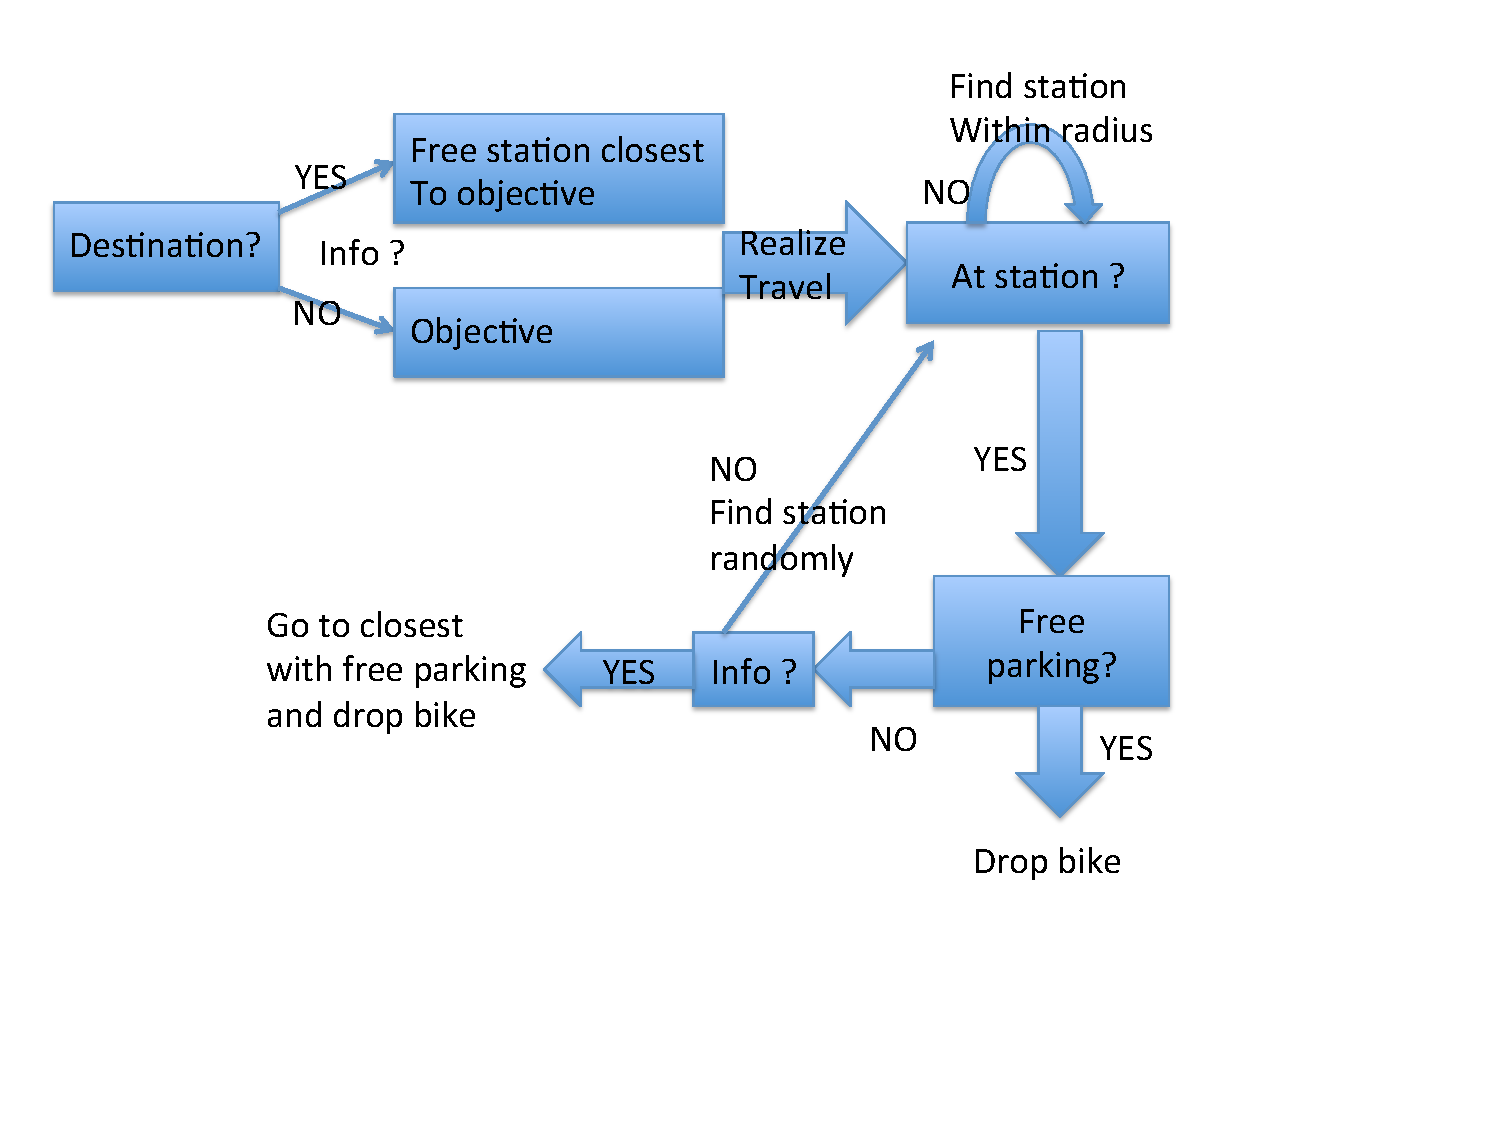
\includegraphics[scale=0.28]{figures/flowchart.pdf}
\caption{\footnotesize Flowchart of the decision process of bikers, from the start of their travel to the drop of the bike.}
\label{fig:1}

\end{wrapfigure}%


\paragraph{Formalisation}

The street network of the area is an euclidian network $(V\subset\mathbb{R}^{2},E\subset V\times V)$
in a closed bounded part of $\mathbb{R}^{2}$. The time is discretized
on a day, so all temporal evolution are defined on $T=[0,24]\cap\tau\mathbb{N}$
with $\tau$ time step (in hours). Docking stations $S$ are particular
vertices of the network for which constant capacities $c(s\in S)$
are defined, and that can contain a variable number of bikes $p_{b}(s)\in\{0,\ldots,c\}^{T}$.
We suppose that temporal fields $O(x,y,t)$ and $D(x,y,t)$ are defined,
corresponding respectively to probabilities that a given point at
a given time becomes the expected departure (resp. the expected arrival)
of a new bike trip, knowing that a trip starting (resp. arriving) at that time exists. Boundaries conditions
are represented as a set of random variables $(N_{I}(i,t))$.
For each possible entry point $i\in I$ ($I\subset V$ is a given
set of boundaries points) and each time, $N_{I}(i,t)$ gives the number
of bikes trips entering the zone at point $i$ and time $t$. For
departures, a random time-serie $N_{D}(t)$ represents the number
of departures in the zone at time $t$. Note that these random variables
and probabilities fields are sufficient to built the complete process
of travel initiation at each time step. Parametrization of the model
will consist in proposing a consistent way to construct them from
real data.

Docking stations are fixed agents, only their functions $p_{b}$ will
vary through time. The other core agents are the bikers, for which
the set $B(t)$ is variable. A biker $b\in B(t)$ is represented
by its mean speed $\bar{v}(b)$, a distance $r(b)$ corresponding to its ``propensity to walk'' and a boolean $i(b)$ expressing the capacity of having access to information on the whole system at any time (through a mobile device and the dedicated application for example). The initial set of bikers $B(0)$ is taken empty, as $t=0$ corresponds to 3a.m. when there is approximately no travels on standard days.


We define then the workflow of the model for one time
step. The following scheme is sequentially executed for each $t\in T$,
representing the evolution of the system on a day.

For each time step the evolution of the system follows this process :
\begin{itemize}
\item Starting new travels. For a travel within the area, if biker has information,
he will adapt his destination to the closest station of its destination
with free parking places, if not his destination is not changed.

\begin{itemize}
\item For each entry point, draw number of new traveler, associate to each
a destination according to $D$ and characteristics (information drawn
uniformly from proportion of information, speed according to fixed
mean speed, radius also).
\item Draw new departures within the area according to $O$, associate either
destination within (in proportion to a fixed parameter $p_{it}$,
proportion of internal travels) the area, or a boundary point (travel
out of the area). If the departure is empty, biker walks to
an other station (with bikes if has information, a random one if not)
and will start his travel after a time determined by mean walking
speed and distance of the station.
\item Make bikers waiting for start for which it is time begin their journey
(correspond to walkers for which a departure station was empty at
a given time step before)
\end{itemize}
\item Make bikers advance of the distance
corresponding to their speed. Travel path is taken as the shortest path between origin and destination, as effective paths are expected to have small deviation from the shortest one in urban bike travels~\cite{borgnat2009spatial}.
\item Finish travels or redirect bikers

\begin{itemize}
\item if the biker was doing an out travel and is on a boundary point, travel
is finished (gets out of the area)
\item if has no information, has reached destination and is not on a station, go to a random station
within $r(b)$
\item if is on a station with free places, drop the bike
\item if is on a station with no places, choose as new destination either
the closest station with free places if he has information, or a random
one within $r(b)$ (excluding already visited ones, implying the memory
of agents).
\end{itemize}

\end{itemize}
Fig. \ref{fig:1} shows the decision process for starting and arriving bikers.
Note that walking radius $r(b)$ and information $i(b)$ have implicitly
great influence on the output of the model, since dropping station
is totally determined (through a random process) by these two parameters
when the destination is given.



\subsection{Discrete Choices Extension}

The extension to this agent-based model is the insertion of a Discrete Choice Model at some decision steps by bikers. The more natural was the choice of waiting at a docking station to get a bike when it is empty, or similarly to wait for a free parking place when station is full, instead of moving to the closest station or taking an other mode. We do not consider the last hypothesis, assuming that users necessarily have already made an immutable mode choice.

Formally, choice are waiting $w$ or moving $m$. We denote by $t_w$ waiting time, $d\textquoteright$ distance to go to next station, and $\tilde{d}$ the distance difference to destination.

For bikers with $i(b)=1$, they know exactly distance to closest station, and choice can be made accordingly, following the utilities
\[
U_w(i=1)=\beta_t t_w + \beta_d \tilde{d} + \varepsilon_w
\]
\[
U_m(i=1)=\beta_t \frac{d\textquoteright}{\bar{v}} + \beta_d \tilde{d} + \varepsilon_m
\]
whereas for a biker with no information, terms in $\tilde{d}$ will vanish as he has no information how far he will go, and traveling distance is different (in that case, user only check the average lost time) :
\[
U_w(i=0)=\beta_t t_w  + \varepsilon_w
\]
\[
U_m(i=0)=\beta_t \frac{\bar{d}}{\bar{v}} + \varepsilon_m
\]

It could be the object of further work to propose the addition of an ``exhaustion\textquoteright \textquoteright term, expressing the reluctance of the user to bike more. Also, risk aversion is not taken into account for uninformed users.

The integration of a nested logit including the choice of use of information if it is available might be interesting, but not necessarily efficient in our method as it would add too many parameters, weakening the calibration procedure.

The extension was implemented and code adapted in order to be able to estimate the two DC parameters we are interested in, i.e. $\beta_t$ and $\beta_d$.


\section{Inference of Unknown Parameters by Model Calibration}


\subsection{Extended Calibration Procedure}

The calibration is done with objective to minimize the error on real data for load factor : if we note $(lf(s,t))_{s\in S,t\in T}$ real time-series, it is defined for the $k$-th realization of the model as 
\[
E(k)=\frac{1}{\left|S\right|\left|T\right|}\sum_{t\in T}\sum_{s\in S}\left(\frac{p_{b}(s,t)}{c(s)}-lf(s,t)\right)^{2}
\]
and we want to minimize the empirical mean on many realization $E=<E(k)>_k$.

Parameter space contains
\begin{itemize}
\item $\bar{r}$ mean walking radius of bikers
\item $p_i$ probability to have information
\item $\sigma$ kernel size for fields inference
\item DC parameters $\beta_t,\beta_d$
\end{itemize}

Dimension is too huge for a systematic grid exploration. We use first results of section 3 to have bounds on DC parameters and significantly reduce search size. We assume $\beta_t \sim \beta_{t_B}$ and $\beta_d \sim \beta_{D}$ so we get $\beta_d \in [-0.06,0]$ and $\beta_{t}\in [-0.25,-0.15]$. Other parameters can be handily bounded : $\bar{r}\in [0,1000],\sigma \in [50,500]$ and $p_i\in [0.3;0.7]$.

We build then a grid of size $10^5$ within this bound and we follow a standard gradient descent for calibration. Fig.\ref{fig:calib} shows examples of projected surfaces on subspaces. Among some dimension, behavior is chaotic and leaves less chances for the classic descent to work, so we add a touch of simulated annealing to help convergence towards an hypothetical global minimum. Empirically, we obtain roughly 76\% of convergence to a small region, that is with 95\% confidence intervals (normal hypothesis) $(\bar{r},p_i,\sigma,\beta_t,\beta_d)=(238\pm 51,0.67\pm 0.08,321\pm 69,-0.05 \pm 0.01, -0.16\pm 0.02)$. We have this way inferred unknown DC parameters, learning that people are less reluctant to move than expected.



\begin{figure}
\label{fig:calib}
\centering
\subfloat[Response surface along $(\sigma,p_i)$ dimensions.]{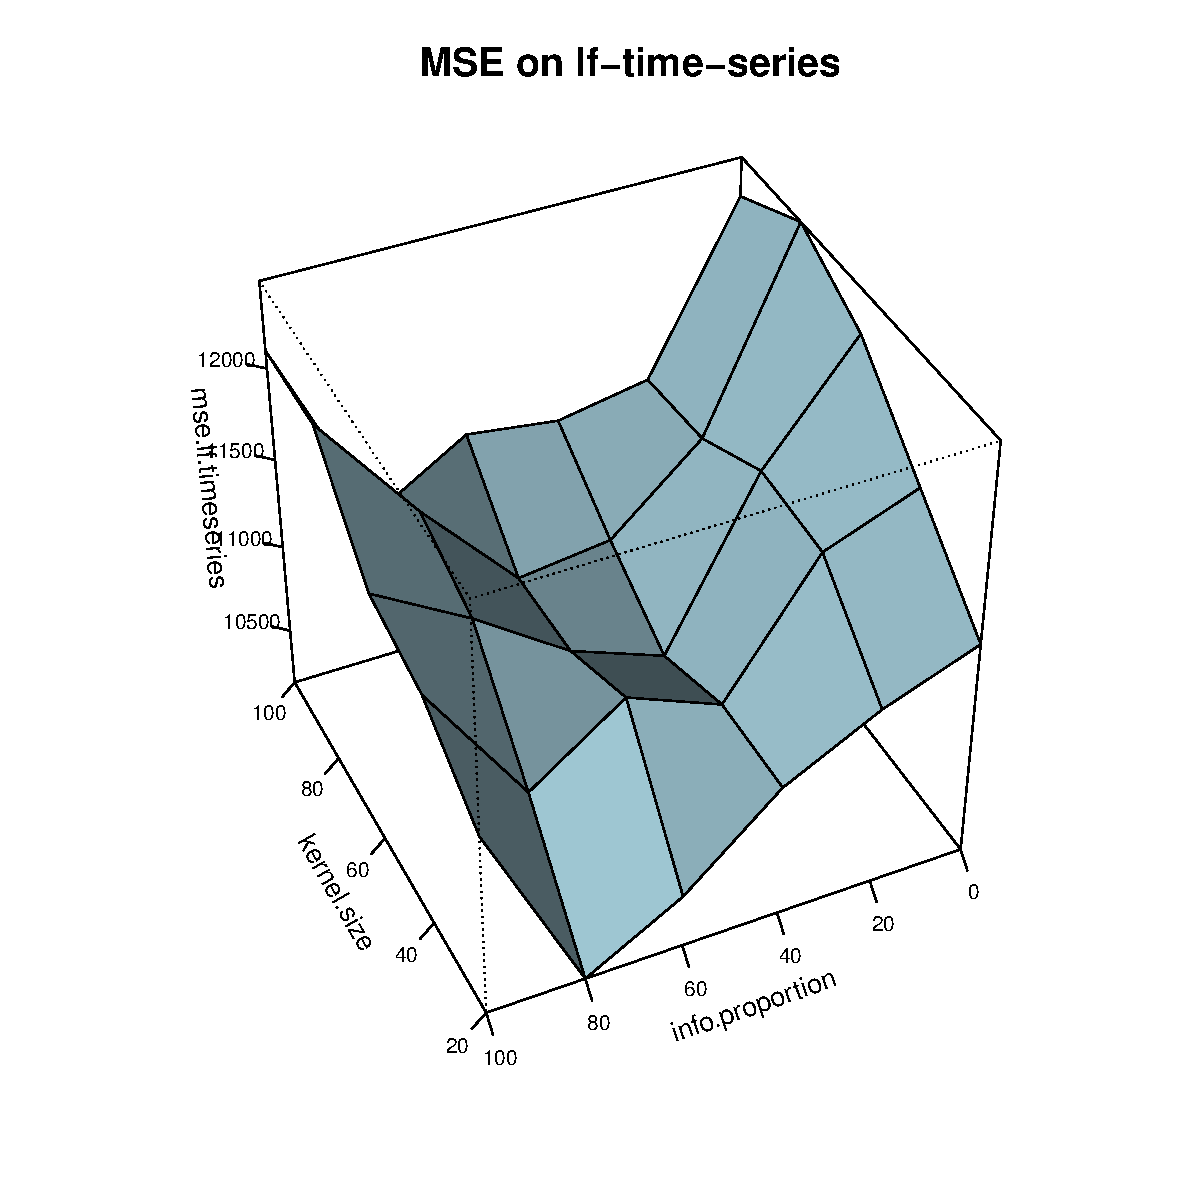
\includegraphics[scale=0.3]{figures/calib3d}}
\hfill{}\subfloat[More chaotic response surface along $(\beta_d,\beta_t)$ (rescaled).]{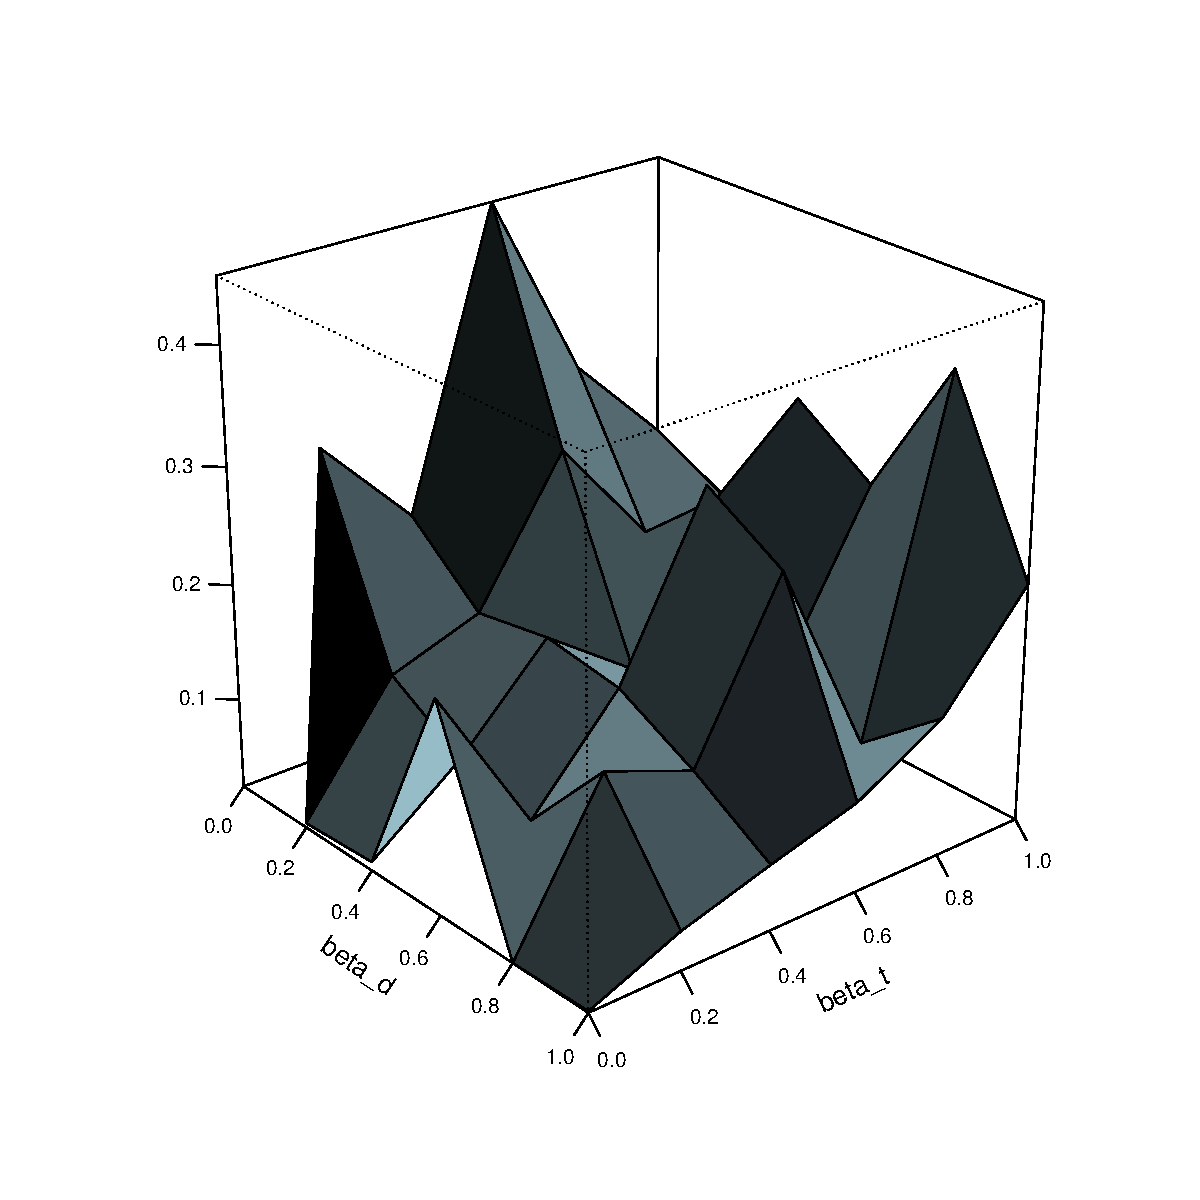
\includegraphics[scale=0.3]{figures/calib_chaos}}
\caption{Example of Mean-square error response surfaces, obtained with $K=100$ repetitions for each combination of parameters. As some parameters allow a regular, almost convex behavior, ideal for simplex calibration, other give chaotic landscapes.}
\end{figure}

\subsection{Towards calibration stability assessment through Large-Deviations functions simulation}

A crucial issue in the proposed calibration procedure is the non-precise knowledge of the behavior of the response surface around the area where parameters seems to give the best results. However, the algorithm did not necessarily converge, and it is difficult to extract statistics because of the rather chaotic geometry along some dimensions (mean behavior on a precise point has no meaning if trajectories are sensitive to infinitesimal disturbances). To tackle the question of the accuracy of the calibration, we propose a novel method inspired from recent works in statistical physics that is the determination of large deviation functions.

Considering a stochastic system where ``extreme\textquoteright \textquoteright event (regarding a given observable, that we can isomorphically consider as an activity $K$) occur in exponentially decreasing probabilities, one can compute its large-deviations function that is linked to the rate of divergence to extreme configurations \cite{touchette2009large}.

Our system will be the model within its parameter space, a configuration given by parameter values, and dynamics following MSE gradient and simulated annealing.

\paragraph{Markov formalism and cloning algorithm}

We place ourselves in the continuous-time Markov chains formalism for describing the system. We consider the set of configurations $\{\mathcal{C}\}$ and the corresponding transition rates between states $W(\mathcal{C}\rightarrow\mathcal{C}'$). We have the master equation for probabilities in time, with the escape rate of a state $r(\mathcal{C})=\sum_{\mathcal{C}'\neq\mathcal{C}}W(\mathcal{C}\rightarrow\mathcal{C}')$
\[
\partial_{t}P(\mathcal{C},t)=\sum_{\mathcal{C}'\neq\mathcal{C}}W(\mathcal{C}'\rightarrow\mathcal{C})P(\mathcal{C}',t)-r(\mathcal{C})P(\mathcal{C},t)
\]

In the case of our system, even gradient of MSE is stochastic as we estimate an empirical gradient on $K$ realizations of the model, therefore escape rate will be empirically calculated at each step, as transition rates. One stays if $ || \vec{grad}E||<\varepsilon$ a given threshold (we take $\varepsilon =1$). One jumps to neighbor states with probabilities linear in component contribution. Finally, one jumps further with a probability $\alpha \cdot Var_R(|| \vec{grad}E||)$ where the variance is taken on a fixed radius $R$ (we take $R=100$ and $\alpha = 0.05$) (probabilities are then normalized). Activity is taken as the mean distance to the expected convergence point.

With the calculation of rates, we can implement the cloning algorithm proposed in \cite{lecomte2007numerical,tailleur2009simulation} (discrete space, discrete time). The idea exploited in the cloning algorithm is to use population dynamics to obtain biased selection of large deviations that could not have been observed in standard runs. The large deviation function $\psi$ is defined, for $s$ conjugated with the activity $K$, by $<e^{-sK}>\sim e^{t\psi(s)}$ where the mean is on all histories.

One has then the $s$-modified master equation for the transformed probabilities $\hat{P}(\mathcal{C},s,t)$, with only the modified rates:

\[
\partial_{t}P(\mathcal{C},s,t)=\sum_{\mathcal{C}'\neq\mathcal{C}}W_{s}(\mathcal{C}'\rightarrow\mathcal{C})P(\mathcal{C}',t)-r(\mathcal{C})P(\mathcal{C},t)
\]


Introducing the $s$-modified escape rate $r_{s}(\mathcal{C})=\sum_{\mathcal{C}'\neq\mathcal{C}}W_{s}(\mathcal{C}\rightarrow\mathcal{C}')$, one can rewrite the above equation as a Markov dynamic with a new escape rate $\delta r_{s}=r_{s}-r$, that we will consider as a cloning rate: if copies of the system evolve in parallel following the new Markov dynamic, and are cloned at rate $\delta r_{s}$, one can show that the size of the population follows the first master equation so one can evaluate $\psi$ by evaluating the linear growth coefficient of the logarithm of population size at large time (detailed in \cite{lecomte2007numerical}). One can also calculate the average of activities on histories, which is of interest for our question.

The algorithm was modified from the open python implementation provided by authors of \cite{tailleur2009simulation}. The calculation of $E$ and its gradient was done through a system call to headless Netlogo running the ABM. First result of curves for $\psi$ and the activity are shown in figure 8 but results are too fuzzy yet to have a clear conclusion on the stability of the calibration. We have however proposed an interesting method that would deserve further exploration and developments.


\begin{figure}
\label{fig:cloning}
\subfloat[$\psi(s)$ for $K=20...100$]{\includegraphics[scale=0.7]{/Users/Juste/Documents/Cours/TheoreticalAnalysisComplexSystems/Project/Results/Cloning/psi}}
\hfill{}
\subfloat[Mean activity for $K=20...100$]{\includegraphics[scale=0.7]{/Users/Juste/Documents/Cours/TheoreticalAnalysisComplexSystems/Project/Results/Cloning/activityspositive}}
\caption{Large-deviation function and mean deviation from minimum, drawn for different values of $K$ number of repetitions. As expected, growing $K$ diminishes the number of deviating events, i.e. stabilize the surfaces. We can conclude than over $K=60$ we have a quite satisfying convergence as $\psi$ vanishes quickly.}
\end{figure}



\section{Conclusion}

Despite the fail on precise survey conception and administration, we turned over the research question towards a less practical but rather interesting methodological and theoretical question : how can we infer missing data or parameters from poor and incomplete data. To answer that, we elaborated a complicated process allowing to reconstruct dynamics of the system by coupling statistical analysis (field inference) with agent-based modeling. This hybrid model can be extended and use to indirectly determine discrete choice parameters by model calibration, allowed by a first rough DC modeling used to obtain a bound on parameters. Finally, we propose a novel method to study the stability of the calibration, using ideas from statistical physics especially numerical calculation of large-deviation functions through a cloning algorithm, opening research paths although it was not directly conclusive.

Further work should first focus on a better junction between all parts of the project, and robustness reinforcement for each single part. Other point mentioned in text can of course be taken as independent developments.


%%%%%%%
%% Biblio
%%%%%%%
\newpage

\bibliographystyle{apalike}
\bibliography{/Users/Juste/Documents/Cours/PIL/DiscreteChoicesBikeSharing/Biblio/bikesDiscreteChoices,/Users/Juste/Documents/ComplexSystems/Biblio/Bibtex/global,/Users/Juste/Documents/ComplexSystems/Biblio/Culture/Bibtex/culture,/Users/Juste/Documents/ComplexSystems/CityBikes/Biblio/bibtex,/Users/Juste/Documents/Cours/TheoreticalAnalysisComplexSystems/Project/Biblio/biblio,/Users/Juste/Documents/ComplexSystems/Misc/DynamiteSSchool2014/Biblio/dynamite}





%%%%%%%%%%%%%%
%% Templates
%%%%%%%%%%%%%%



%%%%%%%%%%%%%%%%%%%%
%% EPJH Fig Template
%%%%%%%%%%%%%%%%%%%%




%\begin{figure}[h]
%\centering
% Use the relevant command for your figure-insertion program
% to insert the figure file.
% For example, with the option graphics use
%\resizebox{0.75\columnwidth}{!}{%
%  \includegraphics{fig1.eps} }
%\caption{Please write your figure caption here.}
%\label{fig:1}       % Give a unique label
%\end{figure}
%


%%%%%%%%%%%%%%%%%%%%
%% EPJH Tab templates
%%%%%%%%%%%%%%%%%%%%

% For tables use
%\begin{table}[h]
%\centering
%\caption{Please write your table caption here.}
%\label{tab:1}       % Give a unique label
% For LaTeX tables use
%\begin{tabular}{lll}
%\hline\noalign{\smallskip}
%first & second & third  \\
%\noalign{\smallskip}\hline\noalign{\smallskip}
%number & number & number \\
%number & number & number \\
%\noalign{\smallskip}\hline
%\end{tabular}
%\end{table}
%


% the bibliography -> not needed [bibtex]

%\begin{thebibliography}{}
% and use \bibitem to create references � ONLY ONE reference by item
% Format for Journal Reference
%\bibitem[Albert 1999]{RefJ} Author. year. Title. \textit{Journal} \textbf{Volume} (number): page numbers
% Format for books
%\bibitem[Arthur 2010]{RefB}
%Author. year. \textit{Title}. Publisher, place, page numbers
% etc
%\end{thebibliography}

\end{document}

% end of file template.tex


